\documentclass{article}
\usepackage{graphicx}
\begin{document}
\title{ُSeyed Ahmad Mousavi Zadeh - 403522145}

\section{Git and GitHub}

\subsection{Repository Initialization and Commits}
برای شروع پروژه:
\begin{enumerate}
    \item یک مخزن جدید در GitHub ایجاد کنید.
    \item مخزن را با دستور زیر کلون کنید:
    \begin{verbatim}
    git clone <URL>
    cd <repository-name>
    \end{verbatim}
    \item فایل‌ها را اضافه کرده و کامیت کنید:
    \begin{verbatim}
    git add .
    git commit -m "Initial commit"
    git push origin main
    \end{verbatim}
\end{enumerate}
\subsection{GitHub Actions for LaTeX Compilation}
برای تنظیم \textbf{GitHub Actions} مراحل زیر را انجام دهید:
\begin{enumerate}
    \item پوشه \texttt{.github/workflows} را ایجاد کنید.
    \item یک فایل \texttt{latex-build.yml} بسازید:
    \begin{verbatim}
    name: Build LaTeX Document
    on:
      push:
        tags:
          - '*'
    jobs:
      build:
        runs-on: ubuntu-latest
        steps:
          - name: Checkout repository
            uses: actions/checkout@v2
          - name: Setup LaTeX
            uses: xu-cheng/latex-action@v2
            with:
              root_file: main.tex
              compiler: pdflatex
    \end{verbatim}
\end{enumerate}
\section{Exploration Tasks}

\subsection{Vim Advanced Features}
ویژگی‌های پیشرفته Vim:
\begin{itemize}
    \item \textbf{ماکروها:} ضبط دستورات با زدن \texttt{q} و تکرار با زدن \texttt{@}.
    \item \textbf{پلاگین‌ها:} استفاده از پلاگین‌های معروف مانند \texttt{vim-fugitive} و \texttt{NERDTree}.
    \item \textbf{حالت ترمینال:} باز کردن ترمینال با دستور \texttt{:term}.
\end{itemize}
\subsection{Memory Profiling}
\subsubsection{Memory Leak}
\textbf{Memory Leak} زمانی رخ می‌دهد که حافظه تخصیص داده شده آزاد نشود و باعث کاهش کارایی سیستم شود.

\subsubsection{Valgrind}
ابزار \textbf{Valgrind} به شناسایی مشکلات حافظه و رفع \textbf{Memory Leak} کمک می‌کند.
\subsection{GNU/Linux Bash Scripting}
\subsubsection{fzf}
برای جستجوی تعاملی فایل‌ها:
\begin{verbatim}
fd -e pdf | fzf
\end{verbatim}

\subsubsection{Opening PDFs with Zathura}
برای باز کردن فایل‌های PDF انتخاب شده:
\begin{verbatim}
zathura $(fd -e pdf | fzf)
\end{verbatim}
\begin{figure}[h!]
    \centering
    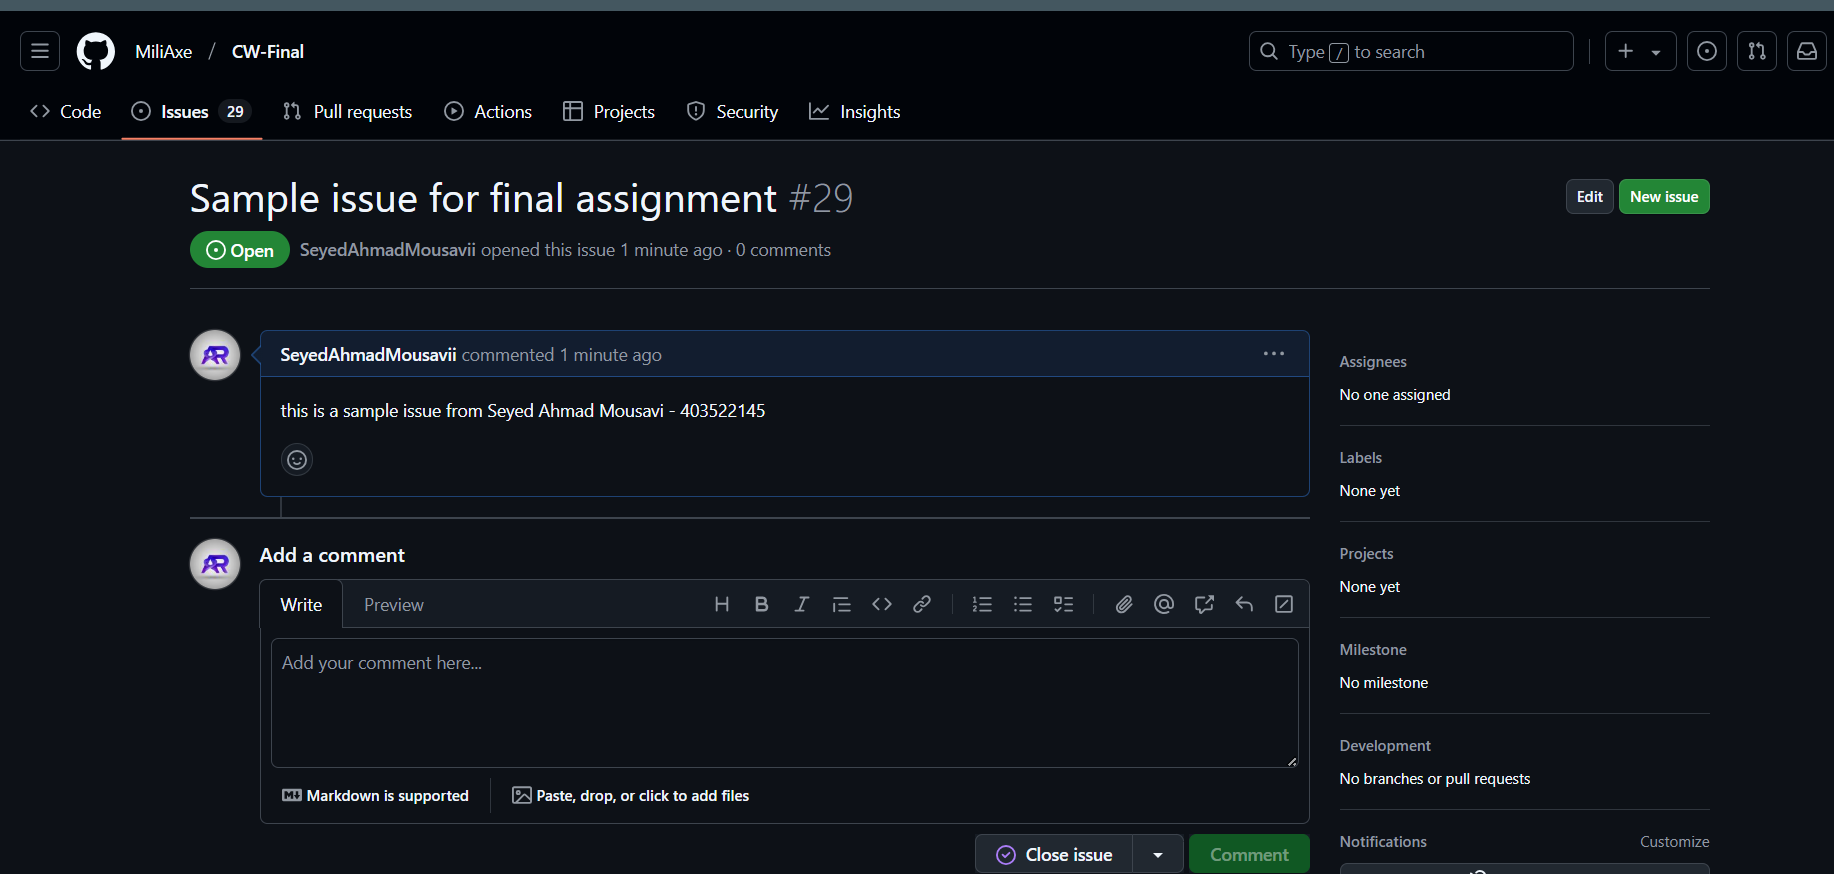
\includegraphics[width=0.5\textwidth]{assets/Screenshot 2025-01-15 233322.png}
    \caption{sample issue}
    \label{fig:example}
\end{figure}

\end{document}